\section{Attacco all'autenticazione delle reti 2G-4G}
Le reti cellulari dal 2G al 4G condividono lo stesso schema architetturale generale, per questo gran parte delle vulnerabilità che vengono
utilizzate negli attacchi di tipo \textit{Denial of Service} sono comuni.
Ci sono numerosi modi per effettuare un attacco DOS all'autenticazione già accennati nella sezione 4.1, in questo capitolo verranno messe in pratica 
nelle reti 2G fino al 4G.\\
Fondamentalmente, in modo da creare un \textit{Denial of Service} nel \textit{Core network} di una rete cellulare tramite una richiesta di autenticazione bisogna forzare
la computazione dei vettori di autenticazione in modo tale da fare spendere risorse computazionali all'infrastruttura cellulare.
Nel momento che un dispositivo si collega alla rete cellulare si possono verificare le seguenti casistiche:
\begin{itemize}
    \item Se il dispositivo ha una SIM valida inizio la procedura di autenticazione.
    \item Se il dispositivo non ha una SIM valida inizio la procedura di autenticazione ma senza consumare abbastanza risorse nel \textit{network}.
    \item Se il dispositivo non ha una SIM la procedura di autenticazione non viene iniziata.
\end{itemize}
Quindi, è chiaro che per effettuare un DOS al sistema di autenticazione degli utenti è necessario disporre o simulare dei dispositivi con delle SIM valide. La validità della SIM è 
in primo luogo controllata dalla presenza di un \textit{International Mobile Subscriber Identity } (IMSI) valido.
Di seguito verranno trattate le principali metodologie per effettuare un DOS al sistema di autenticazione.

\subsection{Botnet}
Il metodo più conosciuto per creare un \textit{Denial of Service} a una rete cellulare è tramite una \textit{botnet}.
In questo modo, l'attaccante ha a disposizione un elevato numero di dispositivi con SIM valida che hanno la possibilità di effettuare massivamente una procedura
di autenticazione causando delle dispendiose computazioni all'interno del \textit{network}.\\
In \cite{measuring-dos} è descritto come effettuare un DDOS a una rete cellulare di tipo 2G/3G in modo da esasperare di richieste il suo componente più critico: l'HLR.
Con 11750 dispositivi infettati è possibile degradare le performance della HLR del 93\%\cite{measuring-dos}, garantendo quindi un quasi totale malfunzionamento dell'infrastruttura.\\
Questa tipologia di attacco è molto pericolosa, e spesso anche la più comune, non è pero esente da diverse problematiche: prima di tutto risulta facilmente rilevabile da un sistema di 
monitoraggio della rete. Inolte, i dispositivi per condurre in maniera efficace un attacco di questo tipo sono un numero molto elevato, sopratutto se si tiene presente che questi dispositivi devono 
appartenere alla stessa zona di competenza della HLR.\\

\subsection{IMSI stealing}
Un metodo alternativo all'utilizzo di una \textit{botnet} è avere a disposizione un \textit{database} di IMSI rubati per effettuare un \textit{flooding} di richieste di autenticazione.\\
Dato che nelle reti 2G-4G l'IMSI viene trasmesso in chiaro al momento dell'autenticazione, in \cite{imsi-catcher} vengono citati i modi più comuni per appropriarsene per poi utilizzarli in un 
attacco.
\begin{figure}[h]
    \centering
    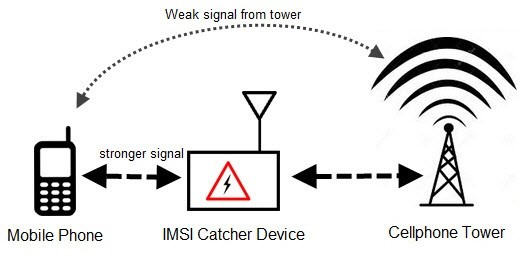
\includegraphics[width=0.5\textwidth]{images/imsi-catcher.jpg}
    \caption{Strumento per rubare IMSI}
\end{figure}\\
Questi dispositivi sono ormai semplici da reperire \textit{online} a un prezzo abbordabile per chiunque. Per rubare l'IMSI si mette in pratica un attacco di tipo \textit{Man In The Middle} (MITM), spesso utilizzato
anche per le intercettazioni da enti governativi.\\
In \cite{dos-imsi} viene illustrato un 



\subsection{Attacco alle reti con dispositivi SIM-less}
\cite{gsm-dos-simless}
In \cite{umts-dos} è descritto un attacco di tipo \textit{Denial of Service} alle reti UMTS, in particolare al
sistema di identificazione degli utenti. \\
Lo studio dmostra che è possibile generare delle onerose computazioni all'interno dell'infrastruttura cellulare senza 
disporre di dispositivi con delle SIM valide. Inoltre, nell'attacco trattato i dispositivi che sono necessari per avere una 
degradazione del servizio sono un numero nettamente minore rispetto allo stato dell'arte, ciò rende la sua realizzazione molto
più accessibile. Con l'inserimento di SIM valide nei dispositivi è possibile ridurre il numero di interfacce UMTS necessarie per compiere 
l'attacco con successo, infatti queste si riducono a qualche centinaio.
Visto il numero contentuto di dispositivi che sono necessari per effettuare l'attacco, si può evitare di usare una \textit{botnet} rendendo l'attacco
molto più stabile e quindi più pericoloso.\\
L'attacco ha come obbiettivo la degradazione di uno dei componenti centrali dell'architettura UMTS: la HLR. Questo componente è il più semplice da 
attaccare poichè avvengono continue interrogazioni durante tutta la fase di autenticazione e identificazione del MS.
Siccome non si tratta di una \textit{botnet} è stata fondamentale l'analisi della capacità dei canali di comunicazione in modo tale da scoprire eventuali
\textit{bottleneck} che minerebbero l'esecuzione dell'attacco.
\begin{figure}[h]
    \centering
    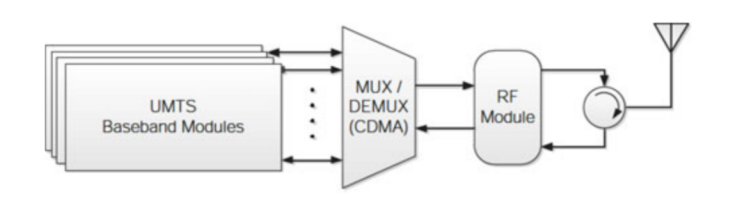
\includegraphics[width=0.5\textwidth]{images/umts-dos-device.png}
    \caption{Dispositivo per l'attacco DOS alle reti UMTS\cite{umts-dos}}
\end{figure}\\
I risultati ottenuti si basano su stime dei tempi di risposta dei componenti architetturali trattati. Questo perchè i vari MNOs non forniscono nessuna 
informazione ufficiale riguardo le \textit{performance}.